\documentclass{article}
\usepackage[paperwidth=538.9mm,paperheight=263mm,margin=0mm]{geometry}
\usepackage{fontspec,xcolor,tikz,graphicx}
\setmainfont{Noto Serif CJK KR}\setsansfont{Noto Sans CJK KR}
\definecolor{navy}{HTML}{14283F}\definecolor{gold}{HTML}{C9A24B}\definecolor{paper}{HTML}{F4EFE3}\definecolor{skyc}{RGB}{196,230,238}
\pagestyle{empty}\setlength{\parindent}{0pt}
% 잠정값: 날개 70mm, 책등 28.9mm(516쪽x0.055+0.5), 도련 3mm -- 교보 사양 확인 후 교체
\newcommand\BL{3mm}\newcommand\WG{70mm}\newcommand\SP{28.9mm}
\begin{document}
\begin{tikzpicture}[remember picture,overlay,x=1mm,y=1mm]
\coordinate (o) at (current page.south west);
\fill[paper] (o) rectangle ([xshift=538.9mm,yshift=263mm]o);
% 좌표(mm): 뒷날개 3~73, 뒷표지 73~255, 책등 255~283.9, 앞표지 283.9~465.9, 앞날개 465.9~535.9
% 앞표지 (위·아래 도련은 색으로 연장)
\fill[skyc] ([xshift=283.9mm]o) rectangle ([xshift=465.9mm,yshift=263mm]o);
\fill[navy] ([xshift=283.9mm]o) rectangle ([xshift=465.9mm,yshift=43mm]o);
\node[anchor=south west,inner sep=0] at ([xshift=283.9mm,yshift=3mm]o) {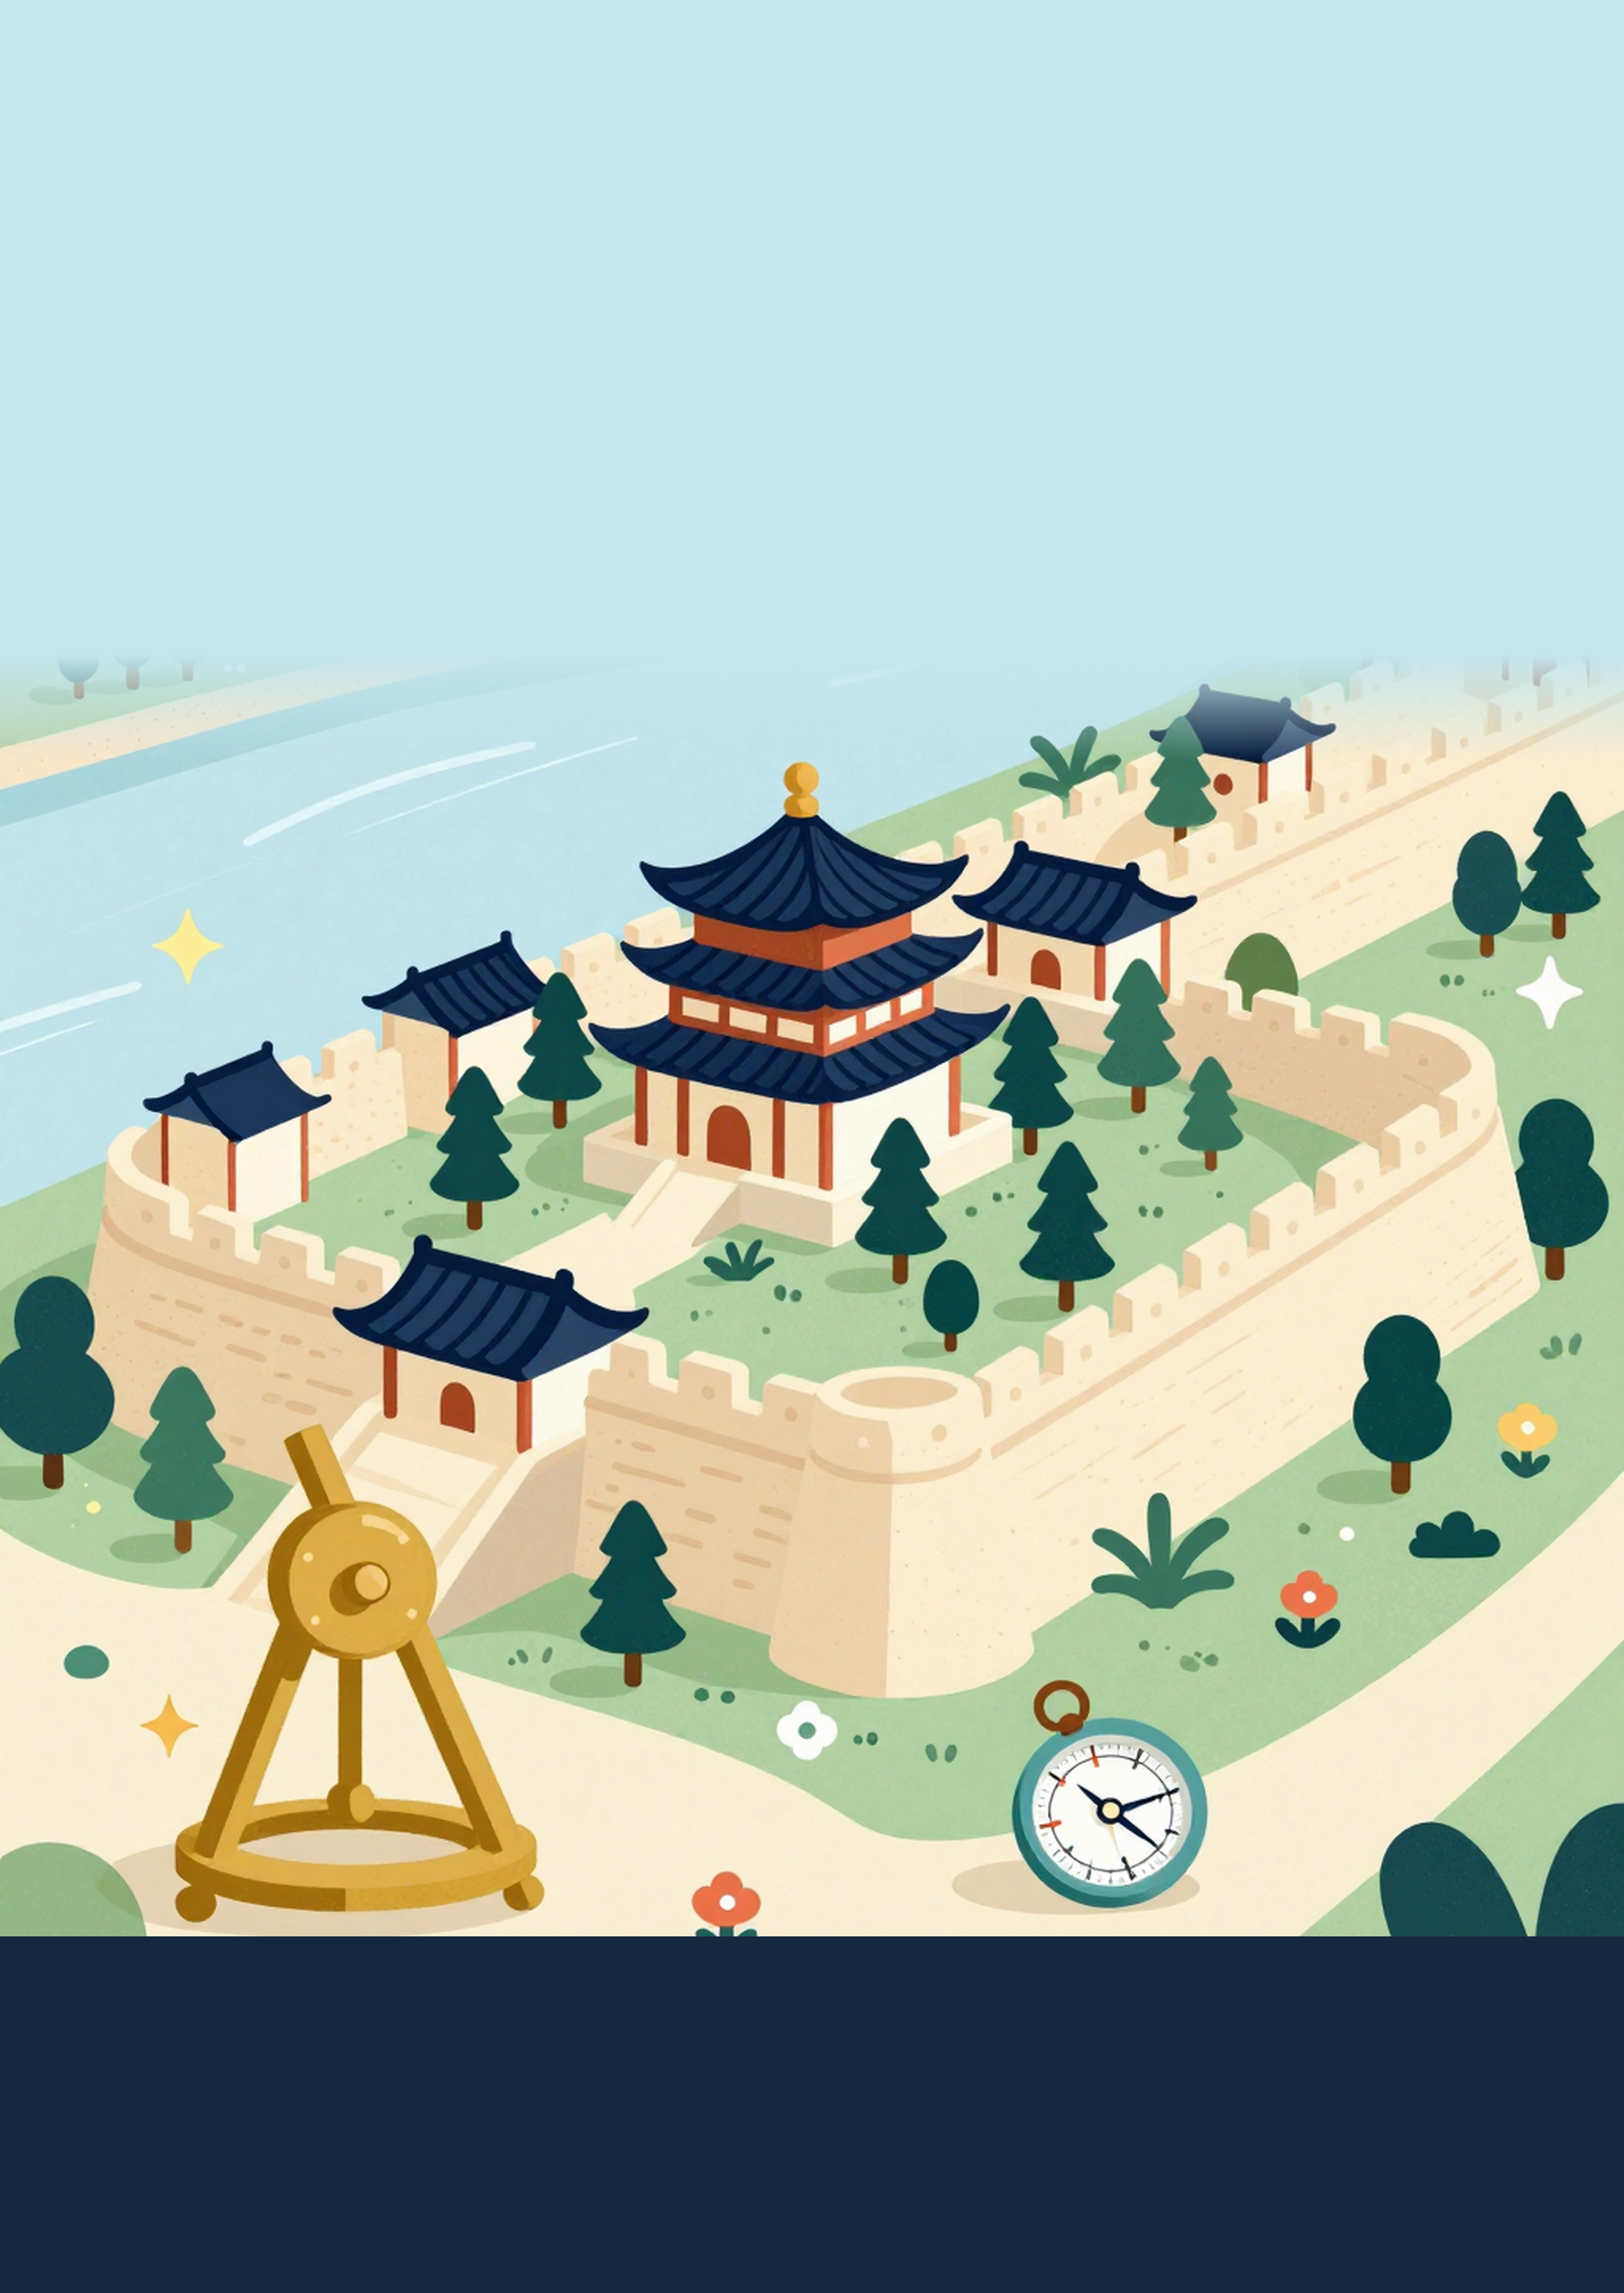
\includegraphics[width=182mm,height=257mm]{cover-v6b-front.png}};
\node[anchor=north west,text=navy,align=left,font=\sffamily\bfseries\fontsize{31}{42}\selectfont] at ([xshift=299.9mm,yshift=249mm]o) {고려 서경(西京)의\\[-2pt]위치를 추정하다};
\node[anchor=north west,text=navy!90!black,align=left,font=\sffamily\bfseries\fontsize{16}{25}\selectfont] at ([xshift=299.9mm,yshift=213mm]o) {여덟 가지 방법으로\\동아시아 고전 지명을\\좌표로 옮기기};
\node[anchor=south west,text=white,font=\sffamily\bfseries\fontsize{22}{26}\selectfont] at ([xshift=299.9mm,yshift=24mm]o) {1권\quad 방법편};
\node[anchor=south west,text=white,font=\sffamily\fontsize{15}{18}\selectfont] at ([xshift=299.9mm,yshift=12mm]o) {이광조 지음};
\node[anchor=south east,inner sep=0] at ([xshift=451.9mm,yshift=13mm]o) {\includegraphics[width=80mm]{logo-dark.pdf}};
% 책등
\fill[navy] ([xshift=255mm]o) rectangle ([xshift=283.9mm,yshift=263mm]o);
\node[rotate=-90,text=white,font=\sffamily\bfseries\fontsize{20}{24}\selectfont,anchor=center] at ([xshift=269.45mm,yshift=148mm]o) {고려 서경(西京)의 위치를 추정하다};
\node[rotate=-90,text=gold,font=\sffamily\fontsize{12}{14}\selectfont,anchor=center] at ([xshift=269.45mm,yshift=48mm]o) {이광조 \quad 과학과영성출판사};
\node[text=white,font=\sffamily\bfseries\Large,anchor=center] at ([xshift=269.45mm,yshift=236mm]o) {1};
% 뒷표지
\node[anchor=north west,inner sep=0] at ([xshift=73mm,yshift=260mm]o) {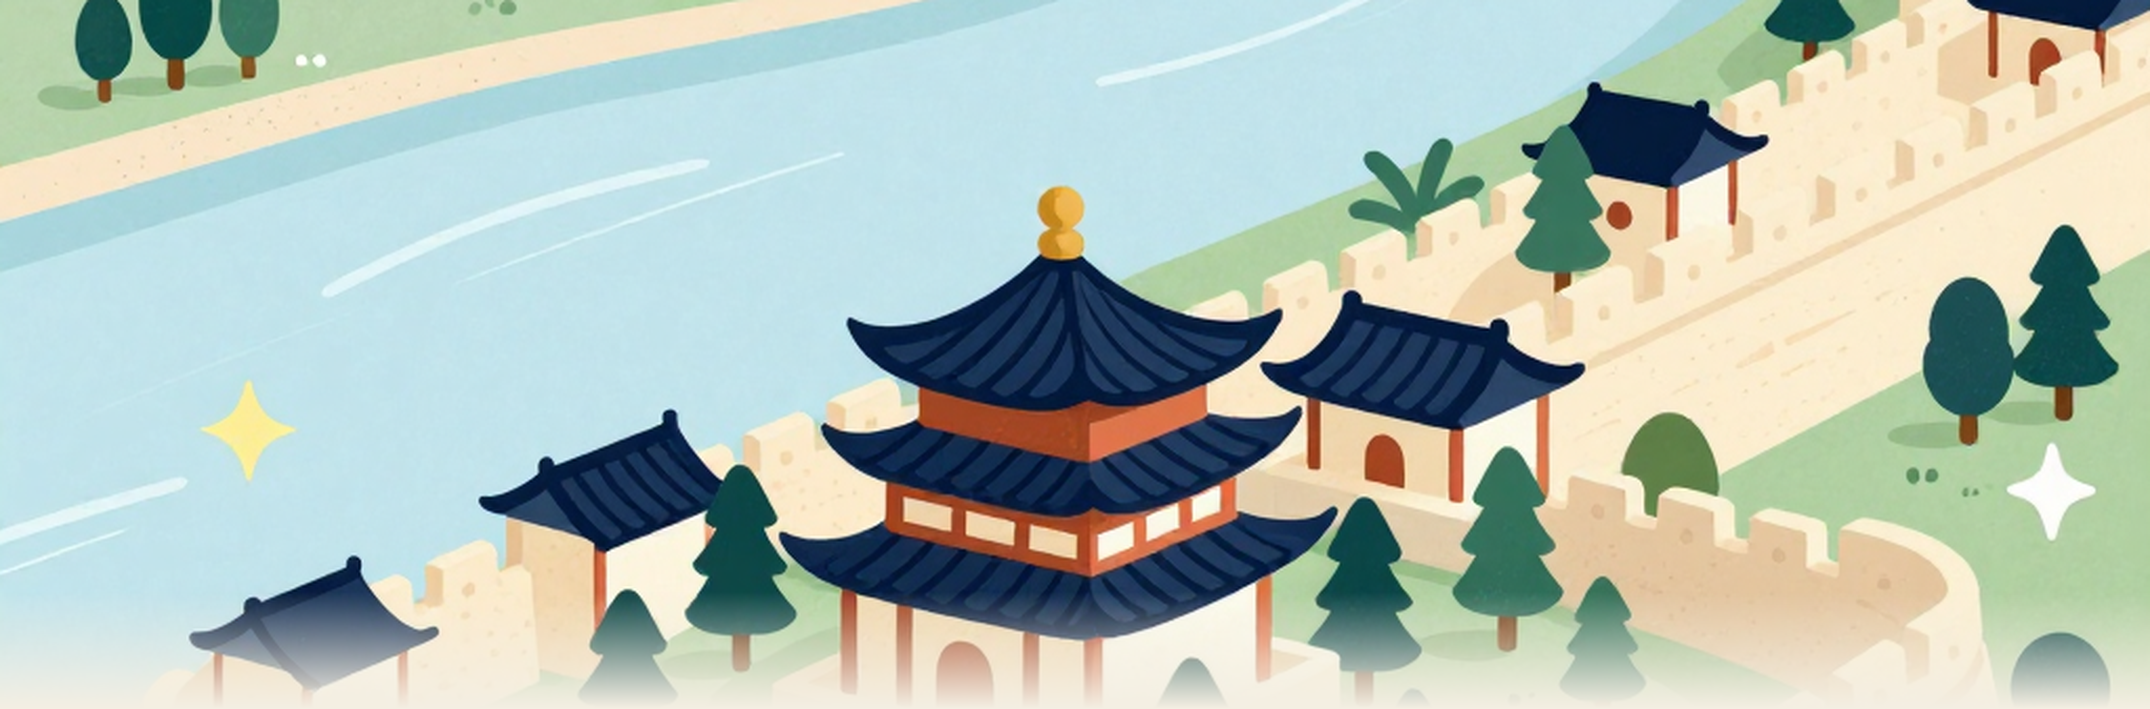
\includegraphics[width=182mm]{cover-v6b-strip.png}};
\node[anchor=north west,text width=146mm,text=navy,font=\sffamily\bfseries\Large] at ([xshift=91mm,yshift=192mm]o) {옛 기록의 ``서쪽으로 십 리''를 지도 위의 점으로};
\node[anchor=north west,text width=146mm,text=black!80,font=\sffamily\normalsize,align=left] at ([xshift=91mm,yshift=172mm]o) {%
이 책은 옛 문헌에 적힌 방위와 거리, 이웃 지명, 산과 강의 서술을 현대 지도의 좌표와 면적으로 바꾸는 여덟 가지 방법을 처음부터 차근차근 설명합니다.\par\vspace{4mm}
제약 전파, 지오레퍼런싱, 베이즈 추정, 최소비용경로 같은 기법을 중학교 2학년 수준의 말로 풀고, 실제 사료의 문장 형태를 본뜬 사례를 입력표부터 결과 해석까지 손으로 계산해 보입니다.\par\vspace{4mm}
고려 서경(西京)의 위치를 추정하는 문제를 끝까지 따라가며, 어떤 증거를 계산에 넣고 어떤 해석은 넣지 않는지를 구분하는 법을 함께 익힙니다.};
\draw[navy,line width=0.5pt,fill=white] ([xshift=197mm,yshift=21mm]o) rectangle ([xshift=237mm,yshift=46mm]o);
\node[text=black!50,font=\sffamily\tiny,align=center] at ([xshift=217mm,yshift=33.5mm]o) {ISBN 바코드 자리\\(ISBN 부여 후 삽입)};
\node[anchor=south west,inner sep=0] at ([xshift=91mm,yshift=25mm]o) {\includegraphics[width=76mm]{logo-light.pdf}};
\node[anchor=south west,text=navy,font=\sffamily\small] at ([xshift=91mm,yshift=15mm]o) {www.ssbook.kr\quad contact@ssbook.kr};
% 앞날개: 저자 소개
\node[anchor=north west,text width=54mm,text=navy,font=\sffamily\bfseries\large] at ([xshift=474mm,yshift=244mm]o) {지은이 이광조};
\node[anchor=north west,text width=54mm,text=black!80,font=\sffamily\small,align=left] at ([xshift=474mm,yshift=230mm]o) {%
서울대학교에서 식품영양학 박사학위를 받았다. 한국식품영양연구소 대표이며 통계 분석을 전문으로 한다. 식물성 영양, 단식 생리, 동양의 전통 지식을 현대 과학과 잇는 연구를 약 30년간 해 왔다.\par\vspace{3mm}
『채식치유학』, 『역사속의 채식인』, 『과학과 초월의 길목에서』 등을 썼다.\par\vspace{3mm}
옛 기록 속의 장소를 증거로 따져 지도 위에 옮기는 일에 통계와 계산을 쓰는 방법을 이 책에서 풀어 썼다.\par\vspace{6mm}
\footnotesize 과학과영성출판사\\www.ssbook.kr\\contact@ssbook.kr};
% 뒷날개: 책 소개(썸네일 4개, 세로)
\node[anchor=north west,text width=56mm,text=navy,font=\sffamily\bfseries\large] at ([xshift=10mm,yshift=250mm]o) {함께 읽는 책};
\node[anchor=north west,inner sep=0] at ([xshift=10mm,yshift=240mm]o) {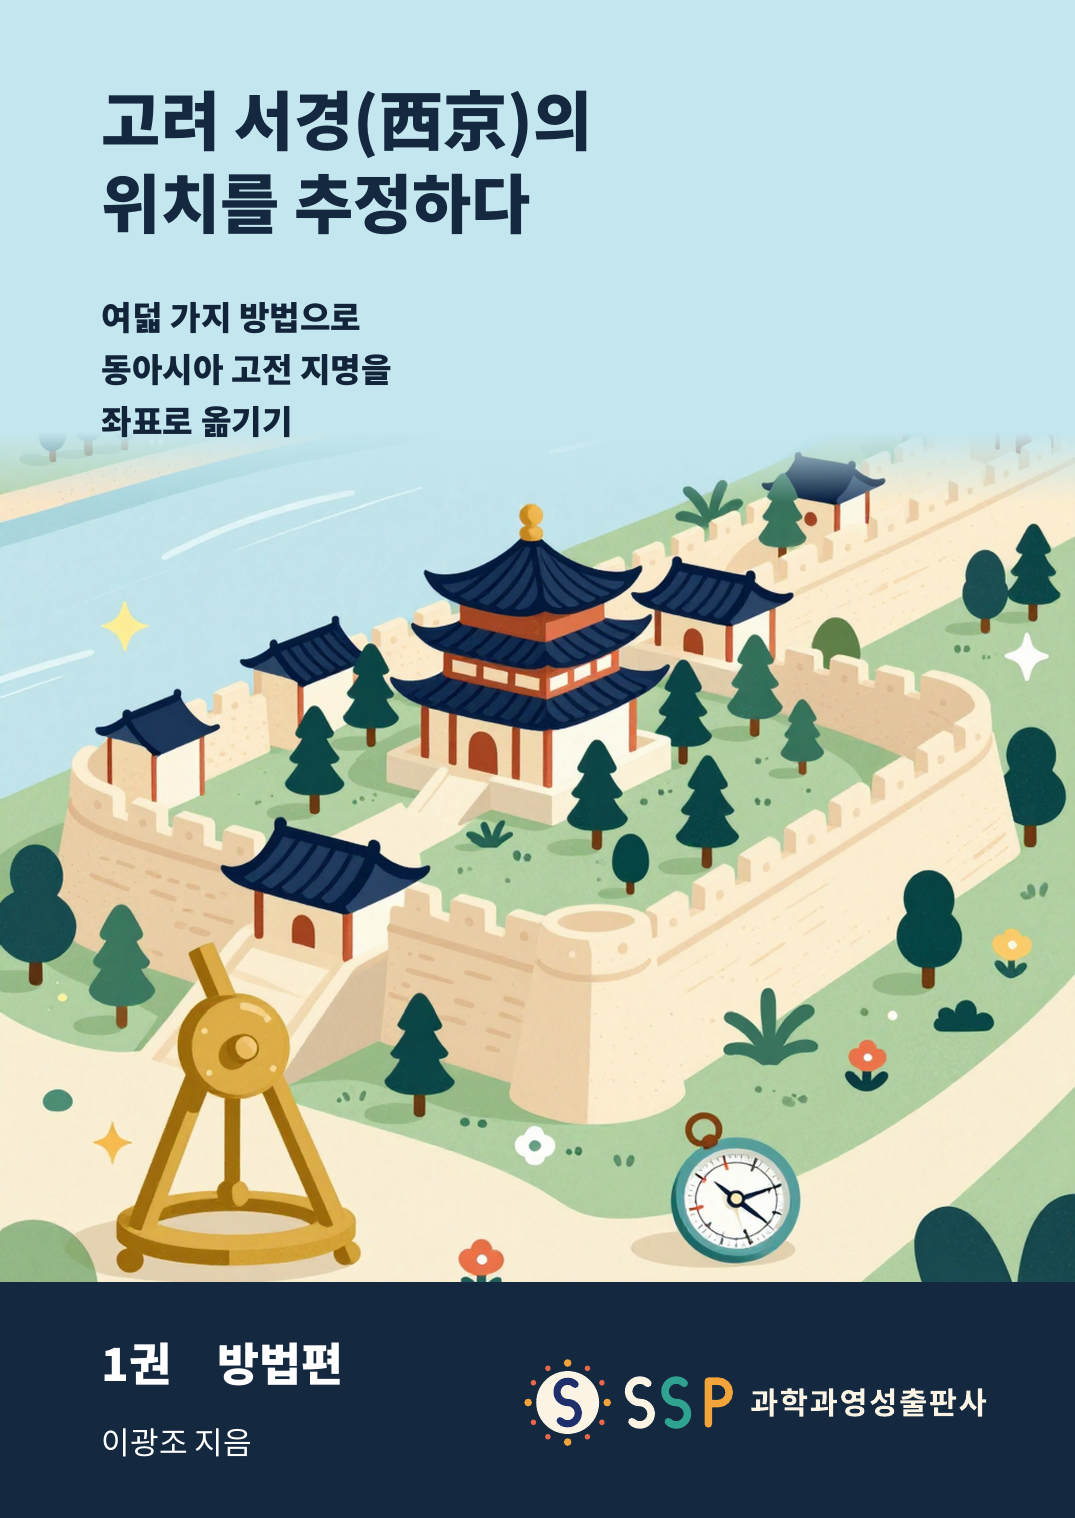
\includegraphics[width=25mm]{thumb1b-1.png}};
\node[anchor=north west,text width=31mm,text=navy,font=\sffamily\bfseries\footnotesize,align=left] at ([xshift=37mm,yshift=240mm]o) {고려 서경(西京)의 위치를 추정하다};
\node[anchor=north west,text width=31mm,text=black!85,font=\sffamily\scriptsize,align=left] at ([xshift=37mm,yshift=231.0mm]o) {\textbf{1권 방법편 (이 책)}\\[1.5pt]옛 기록의 방위, 거리, 이웃 지명을 좌표로 바꾸는 여덟 가지 방법을 처음부터 풀어 쓰고, 서경 하나를 끝까지 손으로 계산해 보입니다. 증거를 층으로 나누어 계산에 넣을 것과 뺄 것을 가르는 법도 익힙니다.};
\node[anchor=north west,inner sep=0] at ([xshift=10mm,yshift=195mm]o) {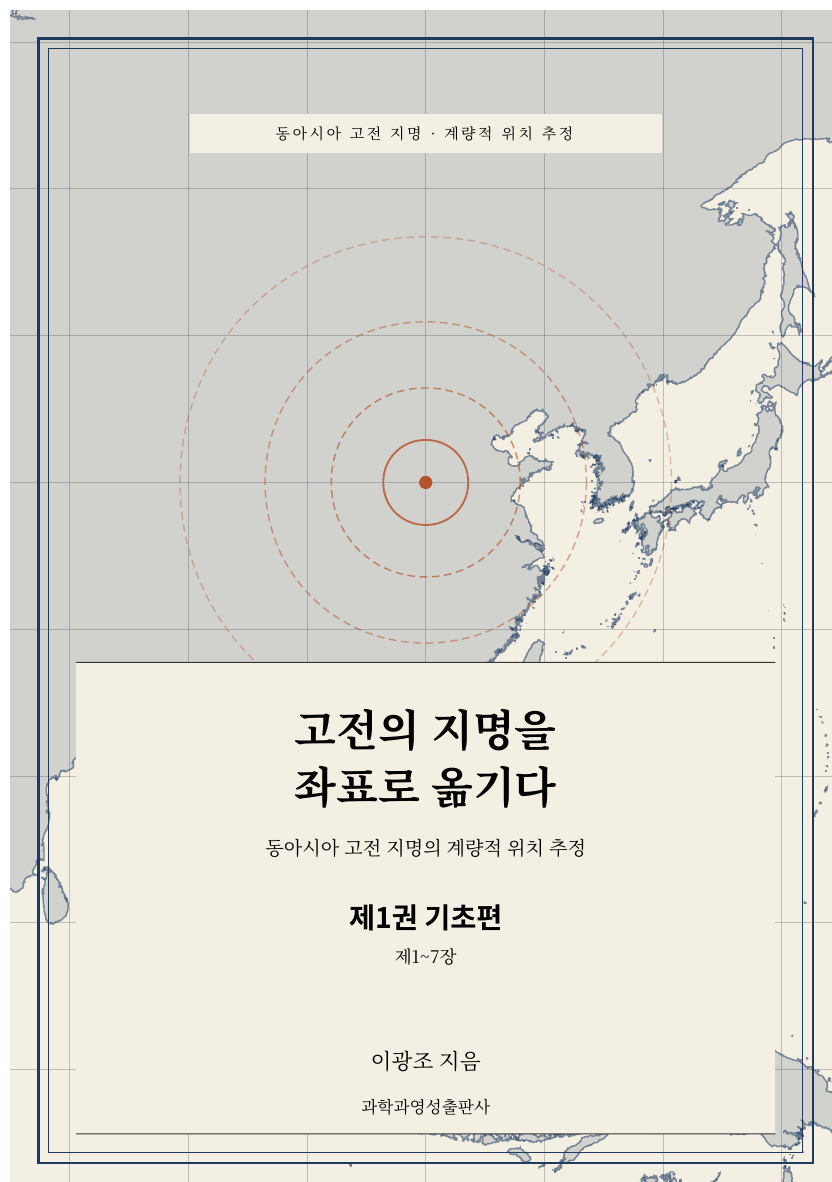
\includegraphics[width=25mm]{gthumb1-001.png}};
\node[anchor=north west,text width=31mm,text=navy,font=\sffamily\bfseries\footnotesize,align=left] at ([xshift=37mm,yshift=195mm]o) {고전의 지명을 좌표로 옮기다};
\node[anchor=north west,text width=31mm,text=black!85,font=\sffamily\scriptsize,align=left] at ([xshift=37mm,yshift=186.0mm]o) {\textbf{1권 기초편 (제1\textasciitilde 7장)}\\[1.5pt]문제 설정, 지도, 수학, 지리, 사료, 레코드와 단위. 이 분야를 처음 접하는 독자가 뒤의 기법을 따라갈 수 있게 바탕을 닦습니다.};
\node[anchor=north west,inner sep=0] at ([xshift=10mm,yshift=150mm]o) {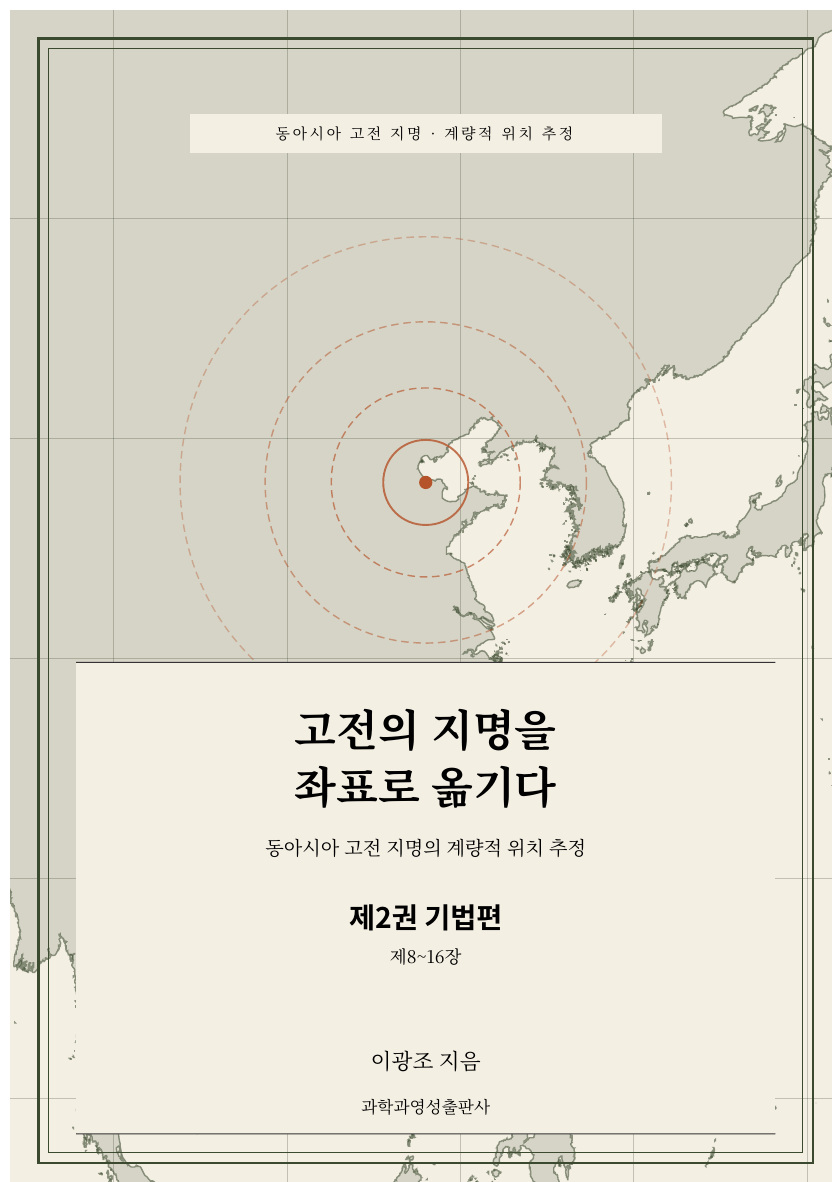
\includegraphics[width=25mm]{gthumb2-001.png}};
\node[anchor=north west,text width=31mm,text=navy,font=\sffamily\bfseries\footnotesize,align=left] at ([xshift=37mm,yshift=150mm]o) {고전의 지명을 좌표로 옮기다};
\node[anchor=north west,text width=31mm,text=black!85,font=\sffamily\scriptsize,align=left] at ([xshift=37mm,yshift=141.0mm]o) {\textbf{2권 기법편 (제8\textasciitilde 16장)}\\[1.5pt]여덟 가지 기법을 하나씩 원리부터 설명하고, 선행연구를 살피고, 같은 문제로 기법을 견주어 봅니다.};
\node[anchor=north west,inner sep=0] at ([xshift=10mm,yshift=105mm]o) {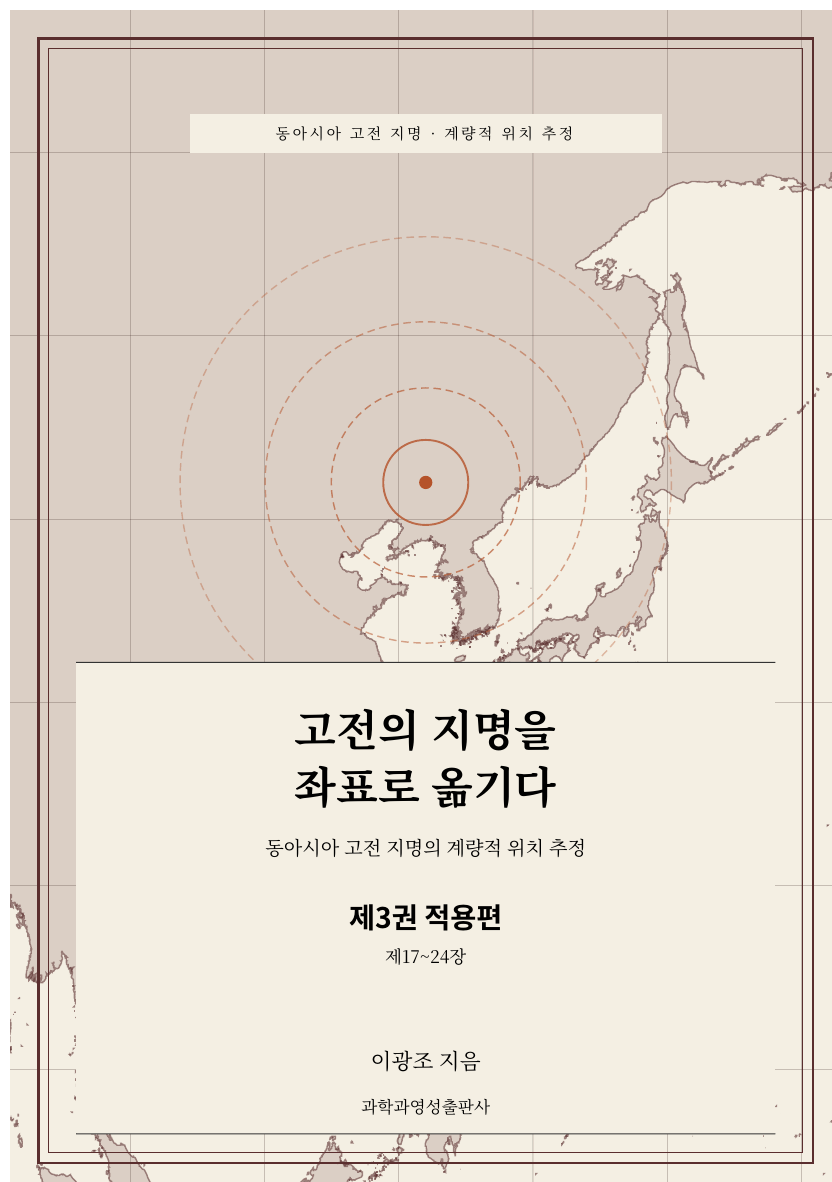
\includegraphics[width=25mm]{gthumb3-001.png}};
\node[anchor=north west,text width=31mm,text=navy,font=\sffamily\bfseries\footnotesize,align=left] at ([xshift=37mm,yshift=105mm]o) {고전의 지명을 좌표로 옮기다};
\node[anchor=north west,text width=31mm,text=black!85,font=\sffamily\scriptsize,align=left] at ([xshift=37mm,yshift=96.0mm]o) {\textbf{3권 적용편 (제17\textasciitilde 24장)}\\[1.5pt]한반도, 요하 유역, 산동과 발해 연안, 만주와 러시아 극동, 서역과 중앙아시아에 적용하고, 통합 추정 방법과 불확실성의 표현, 재현성과 한계를 다룹니다.};
\node[anchor=north west,text width=56mm,text=black!60,font=\sffamily\tiny,align=left] at ([xshift=10mm,yshift=62mm]o) {『고전의 지명을 좌표로 옮기다』는 동아시아 고전 지명의 계량적 위치 추정을 다루는 시리즈입니다. 제목과 구성은 바뀔 수 있습니다.};
% 접는 선(확인용, 인쇄 시 제거)
\foreach \x in {73,255,283.9,465.9} \draw[red!60,line width=0.2pt,dash pattern=on 2pt off 2pt] ([xshift=\x mm]o) -- ([xshift=\x mm,yshift=263mm]o);
\end{tikzpicture}
\end{document}
